\documentclass[a4paper,12pt,twoside]{../includes/ThesisStyle}
\usepackage[utf8]{inputenc}
\usepackage[T1]{fontenc}

\usepackage[left=1.5in,right=1.3in,top=1.1in,bottom=1.1in,includefoot,includehead,headheight=13.6pt]{geometry}\renewcommand{\baselinestretch}{1.05}


% =============================================================================
%\usepackage[sectionbib]{chapterbib}	% Cross-reference package (Natural BiB)
%\usepackage{bibunits}
%\usepackage{natbib}					% Put References at the end of each chapter
\usepackage{algorithm}
\usepackage{alltt}
\usepackage{amsfonts}
\usepackage{amsmath}
\usepackage{amssymb}
\usepackage{cite}
\usepackage{color}
\usepackage{enumerate}
\usepackage{booktabs} % used for \midrule
\usepackage{fancyhdr}					% Fancy Header and Footer
\usepackage{graphicx}
\usepackage{ifthen}
\usepackage{latexsym}
\usepackage{multirow}
\usepackage{rotating}					% Sideways of figures & tables
\usepackage{stmaryrd}
\usepackage{subfigure}
\usepackage{url}         
\usepackage{xspace}
\usepackage[normalem]{ulem} % for \sout
\usepackage{xcolor}
\usepackage{tablefootnote}
\usepackage{pifont}

% =============================================================================

% Table of contents for each chapter
\usepackage[nottoc, notlof, notlot]{tocbibind}
\usepackage{minitoc}
\setcounter{minitocdepth}{1}
\mtcindent=15pt

\setcounter{secnumdepth}{3}
\setcounter{tocdepth}{2}
  
% =============================================================================
% Fancy Header Style Options

\pagestyle{fancy}                       % Sets fancy header and footer
\fancyfoot{}                            % Delete current footer settings

%\renewcommand{\chaptermark}[1]{         % Lower Case Chapter marker style
%  \markboth{\chaptername\ \thechapter.\ #1}}{}} %

%\renewcommand{\sectionmark}[1]{         % Lower case Section marker style
%  \markright{\thesection.\ #1}}         %

\fancyhead[LE,RO]{\bfseries\thepage}    % Page number (boldface) in left on even
% pages and right on odd pages
\fancyhead[RE]{\bfseries\nouppercase{\leftmark}}      % Chapter in the right on even pages
\fancyhead[LO]{\bfseries\nouppercase{\rightmark}}     % Section in the left on odd pages

\let\headruleORIG\headrule
\renewcommand{\headrule}{\color{black} \headruleORIG}
\renewcommand{\headrulewidth}{1.0pt}
\usepackage{colortbl}
\arrayrulecolor{black}

\fancypagestyle{plain}{
  \fancyhead{}
  \fancyfoot{}
  \renewcommand{\headrulewidth}{0pt}
}


% =============================================================================
% Clear Header Style on the Last Empty Odd pages
\makeatletter

\def\cleardoublepage{\clearpage\if@twoside \ifodd\c@page\else%
  \hbox{}%
  \thispagestyle{empty}%              % Empty header styles
  \newpage%
  \if@twocolumn\hbox{}\newpage\fi\fi\fi}

\makeatother

\newenvironment{maxime}[1]
{
\vspace*{0cm}
\hfill
\begin{minipage}{0.5\textwidth}%
%\rule[0.5ex]{\textwidth}{0.1mm}\\%
\hrulefill $\:$ {\bf #1}\\
%\vspace*{-0.25cm}
\it 
}%
{%

\hrulefill
\vspace*{0.5cm}%
\end{minipage}
}

\let\minitocORIG\minitoc
\renewcommand{\minitoc}{\minitocORIG \vspace{1.5em}}


\renewcommand{\epsilon}{\varepsilon}

% centered page environment
\newenvironment{vcenterpage}
	{\newpage\vspace*{\fill}\thispagestyle{empty}\renewcommand{\headrulewidth}{0pt}}
	{\vspace*{\fill}}
	

%=============================================================================

\usepackage{needspace}
\newcommand{\needlines}[1]{\Needspace{#1\baselineskip}}

\usepackage{xcolor}
\definecolor{source}{gray}{0.95}
% source code formatting
\usepackage{listings}
    % global settings for source code listing package
\lstset{
    basicstyle=\ttfamily\small,
    showspaces=false,
    showstringspaces=false,
    captionpos=b, 
    columns=fullflexible}

\lstdefinelanguage{ST}{
    keywordsprefix=\#,
    morekeywords=[0]{true,false,nil},
    morekeywords=[1]{self,super,thisContext},
    morekeywords=[2]{ifTrue:,ifFalse:,whileTrue:,whileFalse:,and:,or:,xor:,not:,by:,timesRepeat:},
    sensitive=true,
    morecomment=[s]{"}{"},
    morestring=[d]',
    escapechar={!},
    alsoletter={., :, -, =, +, <},
    moredelim=**[is][\itshape]{/+}{+/},
    literate=
        {^}{{$\uparrow$}}1
        {:=}{{$\leftarrow$}}1
        {~}{{$\sim$}}1
        {-}{{\sf -\hspace{-0.13em}-}}1  % the goal is to make - the same width as +
        {+}{\raisebox{0.08ex}{+}}1		% and to raise + off the baseline to match V
        , % Don't forget the comma at the end!
    style=STStyle
}
\lstdefinestyle{STStyle}{
    tabsize=4,
    %frame=leftline,
    % frame=bl,
    %framerule=2pt,
    %rulecolor=\color{gray},
    % backgroundcolor=\color{white},
    %backgroundcolor=\usebeamercolor[bg]{listing},
    basicstyle=\ttfamily\small,
    keywordstyle=\bf\ttfamily,
    % stringstyle=\color{orange},
    stringstyle=\mdseries\slshape,
    commentstyle=\it\rmfamily\color{darkgray}, 
    commentstyle=\mdseries\slshape\color{gray},
    %commentstyle=\mdseries\slshape,
    emphstyle=\bf\ttfamily,
    escapeinside={!}{!},
	%backgroundcolor=\color{source},
    %emphstyle={[2]\color{red}},
    %emphstyle={[3]\color{blue}\bf},
    %emphstyle={[4]\color{blue}},
    keepspaces=true
} 

%\lstnewenvironment{javacode}  [1][]{\lstset{language=java,#1}\needlines{#2}}{} 
%\lstnewenvironment{pythoncode}[2][]{\lstset{language=python,#1}\needlines{#2}}{}
\lstnewenvironment{stcode}    [2][]{\lstset{language=ST,#1}\needlines{#2}}{}
\lstnewenvironment{ccode}     [2][]
    {\lstset{language=C,numbers=left,escapechar=\$,numberstyle=\tiny,#1}\needlines{#2}}{}

% ON: I tried to pass the line number options in as arg #1 but it does not work for me
% I also could net get the line numbers to consistently increase
\lstnewenvironment{numstcode} [2][]
    {\lstset{language=ST,numbers=left,numberstyle=\tiny,numbersep=2pt,#1}\needlines{#2}}{}
\lstnewenvironment{numstcodecont} [2][]
    {\lstset{language=ST,numbers=left,numberstyle=\tiny,numbersep=2pt,firstnumber=last#1}\needlines{#2}}{}

\newcommand{\lst}[1]{{\tt #1}}

% In-line code (literal)

% In-line code (latex enabled)
% Use this only in special situations where \ct does not work
% (within Section headings ...):
\newcommand{\lct}[1]{{\textsf{\textup{#1}}}}
% Code environments
\lstnewenvironment{code}{%
	\lstset{%
		% frame=lines,
		frame=single,
		framerule=0pt,
		mathescape=false
	}
}{}

%\renewcommand{\lstlistingname}{Code Example}

% =============================================================================
\newboolean{showcomments}
\setboolean{showcomments}{true}

\ifthenelse{\boolean{showcomments}} {
	\newcommand{\ugh}[1] {\textcolor{red}{\uwave{#1}}}	% please rephrase
	\newcommand{\ins}[1] {\textcolor{blue}{\uline{#1}}}	% please insert
	\newcommand{\del}[1] {\textcolor{red}{\sout{#1}}}	% please delete
	\newcommand{\chg}[2] {								% please change
		\textcolor{red}{\sout{#1}}{\ra}
		\textcolor{blue}{\uline{#2}}}
	\newcommand{\nbc}[3]{								% comment
		{\colorbox{#3}{\bfseries\sffamily\scriptsize\textcolor{white}{#1}}}
		{\textcolor{#3}{\sf\small$\blacktriangleright$\textit{#2}$\blacktriangleleft$}}}

}{
	\newcommand{\ugh}[1]{#1}							% please rephrase
	\newcommand{\ins}[1]{#1}							% please insert
	\newcommand{\del}[1]{}								% please delete
	\newcommand{\chg}[2]{#2}							% please change
	\newcommand{\nbc}[3]{}								% comment
}

% =============================================================================
\usepackage[pagebackref,hyperindex=true]{hyperref}


% Links in pdf
\usepackage{color}
\definecolor{linkcol}{rgb}{0.0, 0.0, 0.0} 
\definecolor{citecol}{rgb}{0.0, 0.0, 0.0} 

% Change this to change the informations included in the pdf file
% See hyperref documentation for information on those parameters
\hypersetup {
	bookmarksopen=true,
	pdftitle="Design and Use of Anatomical Atlases for Radiotherapy",
	pdfauthor="Olivier COMMOWICK", 
	pdfsubject="Creation of atlases and atlas based segmentation", %subject of the document
	%pdftoolbar=false, % toolbar hidden
	pdfmenubar=true, %menubar shown
	pdfhighlight=/O, %effect of clicking on a link
	colorlinks=true,
	pdfpagemode=UseNone,
	pdfpagelayout=SinglePage,
	pdffitwindow=true,
	linkcolor=linkcol,
	citecolor=citecol,
	urlcolor=linkcol
}

% =============================================================================
\newcommand{\figlabel}[1] {\label{fig:#1}}
\newcommand{\chaplabel}[1]{\label{chap:#1}}
\newcommand{\seclabel}[1] {\label{sec:#1}}
\newcommand{\tablabel}[1] {\label{tab:#1}}
\newcommand{\lstlabel}[1] {\label{lst:#1}}

\newcommand{\figref}[1] {Figure~\ref{fig:#1}}
\newcommand{\chapref}[1]{Chapter~\ref{sec:#1}}
\newcommand{\secref}[1] {Section~\ref{sec:#1}}
\newcommand{\tabref}[1] {Table~\ref{tab:#1}}
\newcommand{\lstref}[1] {Listing~\ref{tab:#1}}

\newcommand{\commented}[1]{}

\newcommand{\bs}    {\symbol{'134}} % backslash
\newcommand{\us}    {\symbol{'137}} % underscore
\newcommand{\ttt}[1]{\texttt{#1}}
\newcommand{\ie}    {\emph{i.e.},\xspace}
\newcommand{\eg}    {\emph{e.g.},\xspace}
\newcommand{\etal}  {\emph{et al.}\xspace}
\newcommand{\ns}    {\!\!\!\!} %big negative space
\newcommand{\cnull} {\textbackslash0\xspace}


\newcommand\fix[1]{\nb{FIX}{#1}}
\newcommand\todo[1]{\nb{TO DO}{#1}}
\newcommand\cb[1]{\nbc{CB}{#1}{purple}}
\newcommand\sd[1]{\nbc{SD}{#1}{orange}}
\newcommand\is[1]{\nbc{IS}{#1}{gray}}
\newcommand\gc[1]{\nbc{GC}{#1}{olive}}
\newcommand\ct[1]{\nbc{CT}{#1}{teal}}
\newcommand\md[1]{\nbc{MD}{#1}{blue}}
\newcommand\dc[1]{\nbc{DC}{#1}{green}}

% =============================================================================
\newcommand{\NBFFI}  {Native\-Boost-FFI\xspace}
\newcommand{\NB}  {Native\-Boost\xspace}
\newcommand{\B}   {Benzo\xspace}
\newcommand{\ST}  {Small\-talk\xspace}
\newcommand{\PH}  {Pharo\xspace}
\graphicspath{{.}{../figures/}}

\begin{document}
% =============================================================================
\chapter{Future Work}
\chaplabel{future}
\minitoc
% =============================================================================
\introduction
% =============================================================================

In \chapref{background} we gave an overview of different concepts of reflection and we focused on the main distinction between language-side and \VM-side reflection.
While language-side reflection is very well described in research and rather wide-spread in dynamic languages, the \VM-side counterpart is not.
Up to some extent it is always possible to introspect the \VM at a very basic level.
Tools like \DTrace provide a simple way to instrument a binary.
However, that still does not make the internal structure of the \VM accessible that were available at compilation time.
And the restrictions are even more sever when it comes to \VM-level intercession.
Languages are hardly capable of directly influencing the underlying \VM in a structured way.

In the course of this thesis we presented tools that try to access this special area of \VM-level reflection -- all based on \B, a common framework to activate native code from language-side.

\WF's dynamic primitives are a first step towards modifying \VM behavior from language-side in a rather controlled way.
By bringing the metacircular \VM definition alive in \PH we connect the former static definition to the running artifact.
Modification happens not by injecting basic native instructions but at high-level by modifying and dynamically compiling primitive definitions.

In contrast to \WF we developed \NBJ, a \JIT compiler prototype, that moves the original \VM component to the language-side.
While \NBJ is defined as language-side compiler using familiar coding patterns its \VM interaction is by far not clean.
Unlike the plugins and primitives defined by \WF the \JIT generates native code that is closely integrated into the low-level execution model of the \VM.
As a result \NBJ needs to manually circumvent the current restrictions of the \VM, clearly not an optimal path.

In this chapter we present possible solutions and an early prototype \VM that addresses the limitations we encountered while developing \NB, the \B-based \FFI, \WF and \NBJ.



% =============================================================================
%\newpage
\section{Language-side Improvements}
% =============================================================================
\todo{intro: extend the summary of \chapref{reification}}

% -----------------------------------------------------------------------------
\subsection{Domain Specific Inspectors}
% -----------------------------------------------------------------------------
\todo{More specific Inspectors (Also for VM development)} \\
\todo{Restate the original VM Simulator to provide a smooth VM dev experience}


% -----------------------------------------------------------------------------
\subsection{Barrier Free Low-level Interaction}
% -----------------------------------------------------------------------------
\todo{Provide nice infrastructure for multi-platform low-level interaction} \\
\todo{Provide debugging infrastructure for Benzo}

% -----------------------------------------------------------------------------
\subsection{Virtual CPU an Assembler DSL}
% -----------------------------------------------------------------------------
\todo{small summary of the current shortcomings} \\
\todo{Current State of the Implementation} \\
\todo{Support new Platforms} \\
\todo{Indirect support for simluation and thus better debugging}


% =============================================================================
\section{\VM-level Improvements}
\seclabel{future-vm}
% =============================================================================
\todo{Introduction: Lanugage-side is not enough} \\
\todo{Need to get a onstacle-free VM} \\
\todo{List of requirements for a new VM Infrastructure} \\ 
\todo{Small comparison against the current solution we have with COG}

% -----------------------------------------------------------------------------
\subsection{Introduction}
% -----------------------------------------------------------------------------
\todo{List the current state of the MATE infrastructure}

% -----------------------------------------------------------------------------
\subsection{VM-level Reification}
% -----------------------------------------------------------------------------
\todo{Resulting from the first law of Inspectors, all VM-level objects are reified} \\
\todo{List of typical objects that don't have a reification in COG} \\
\todo{List advantages}

% -----------------------------------------------------------------------------
\subsection{Runtime Reification / Dual Objects}
% -----------------------------------------------------------------------------
\todo{Reuse the same objects for the bootstrap and at runtime inspectors/mirrors} \\
\todo{goes further than the sheer compile-time reification} \\
\todo{accessible from language-side => leads to the following MOP}

% -----------------------------------------------------------------------------
\subsection{Mate Object Model and Runtime MOP}
% -----------------------------------------------------------------------------
\todo{consequence of the runtime reification of the VM introspection => intercession}\\
\todo{Rough Overview of all the Objects currently present in Mate (UMLish)}

% -----------------------------------------------------------------------------
\subsection{Be Native}
% -----------------------------------------------------------------------------
\todo{out of the intercession capabilities follows that we need native support at runtime (see \B)}\\
\todo{that means we need to have decent / better infrasrtucture for native code}\\
\todo{need to be able to achieve what \NBJ didn't manage: compile native methods and hand them over to the \VM}\\
\todo{step towards our implementation in \Mate}


% =============================================================================
\section{\Mate a \VM prototype}
\seclabel{mate}
% =============================================================================

\begin{figure*}[h]
	\begin{adjustwidth}{-10.0in}{-10.0in}
		\centering
		
\includegraphics[width=1.02\textwidth]{mate-logo}
	\end{adjustwidth}
\end{figure*}

\todo{introduction: protoype based on the conclusions presented in the previous sections}\\
\todo{for reasearch mainly but possible long term solution to our \VM problems}

% -----------------------------------------------------------------------------
\subsection{Mate Compiler Outline}
\seclabel{future-mate-compiler}
% -----------------------------------------------------------------------------
\todo{Small Intro: Reuse the bootstrap infrastrucutre at runtime (FFI, JIT...)}

\begin{figure}[H]
\centering
	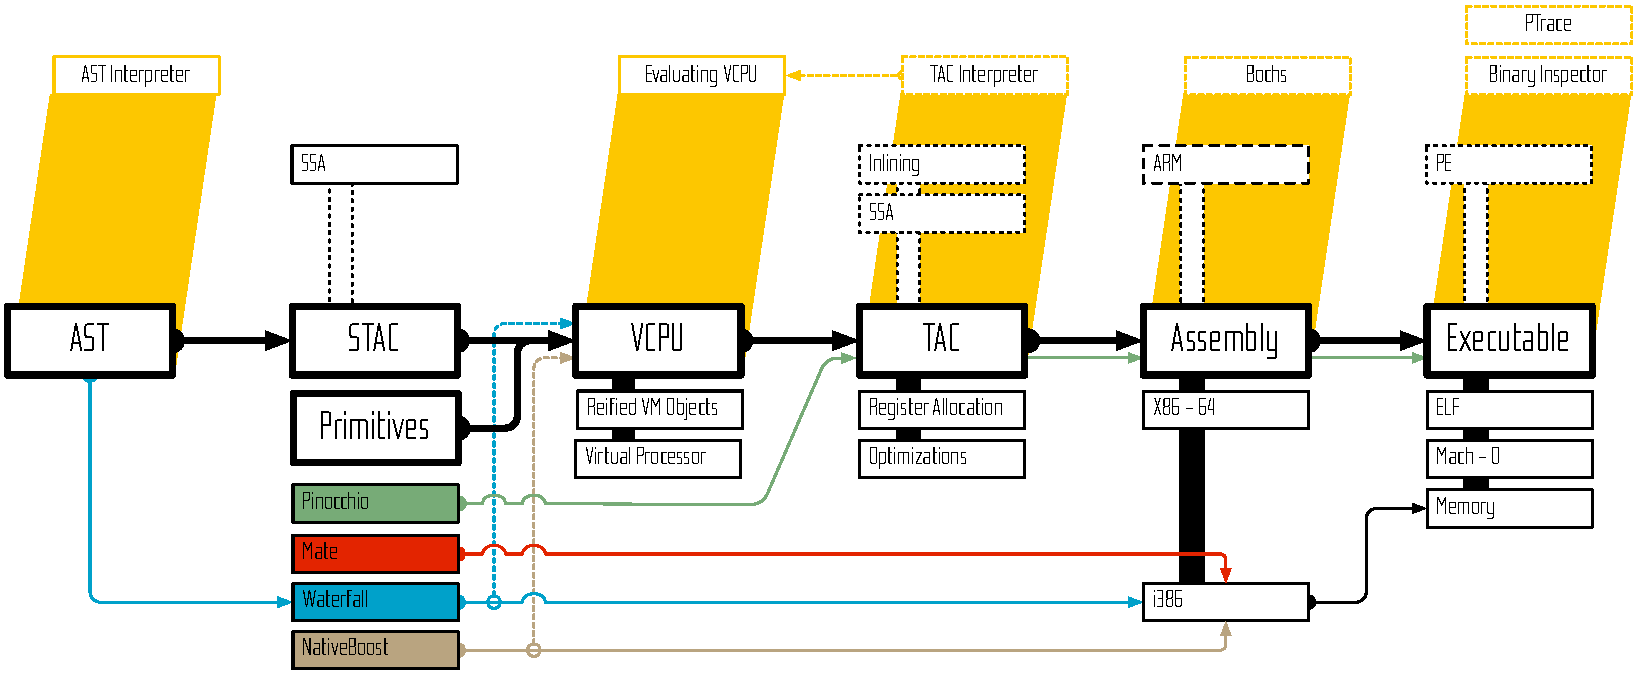
\includegraphics[width=\textwidth]{mate-compilation-toolchain}
\end{figure}

% -----------------------------------------------------------------------------
\subsection{Mate Bootstrap Outline}
\todo{Small Intro: Why Bootstrap and how to use the reified objects}\\
\todo{Compare to Pinocchio (manual approach)}\\
\todo{Work in Progress: Envision the trace-based Bootstrap}


% -----------------------------------------------------------------------------
\subsection{Mate Towards Complete Reflection}
\todo{list possible paths between the 4 quadrants of reflection}\\
\todo{usecase: dynamic gc change}\\
\todo{usecase: dynamic object format influence}\\
\todo{usecase: optimize partial behavior reflection (immutability, proxies)}\\

% -----------------------------------------------------------------------------
\subsection{Related Work}
% -----------------------------------------------------------------------------
\todo{Squeak VM} \\
\todo{Cog} \\
\todo{Pinocchio} \\
\todo{MIST}


% =============================================================================
\section{Reflective Future}
% =============================================================================
% NEW concepts
\todo{Check with GUIDO} \\
\todo{List 3 to 4 different Examples entering the 4th quadrant:}

% -----------------------------------------------------------------------------
\subsection{Accessible VM Components}
% -----------------------------------------------------------------------------
\todo{Access GC Statistics} \\
\todo{Access JIT Statistics for Type Annotations / Tooling}

% -----------------------------------------------------------------------------
\subsection{Interchangeable VM Components}
% -----------------------------------------------------------------------------
\todo{Change GC strategy} \\
\todo{Change JIT Strategy}

% -----------------------------------------------------------------------------
\subsection{Interchangeable Language Semantics}
% -----------------------------------------------------------------------------
\todo{Up to which extent can this be supported?} \\
\todo{Related to VM MOP: How much should be changeable? When?}


% -----------------------------------------------------------------------------
\subsection{Efficient Reflection}
% -----------------------------------------------------------------------------
\todo{Reflectivity at VM-level} \\
\todo{Flatten but don't freeze Reflection/Abstraction}


% =============================================================================
\section{Summary}
% =============================================================================


% =============================================================================
\ifx\wholebook\relax\else
    \end{document}
\fi